All the analysis in this thesis so far have been restricted to the mean-field level. While this is sufficient for qualitative results, it generates very poor quantitative estimates of phase boundaries. In some cases, it can result in entirely incorrect prediction of the existence of certain phases as well. This motivates us to look for better numerical techniques that can allow us to study the system beyond the mean-field level. In this chapter, we will discuss some of these techniques and the difficulties that arise due to the complexity involved in them.

\section{Variational Monte Carlo}
One of the issues with exact diagonalization is that the basis set scales exponentially with the system size. As a result, the memory required simply to represent the wavefunction on a computer quickly grows beyond bounds. This motivates us to look for ways to exploit structure in the wavefunction and find a more compact representation. 
\vspace{0.5cm}\\
The standard scheme in such a case is to guess an ansatz for the wavefunction by leveraging the variational principle. The ground state can then be obtained by tuning the free parameters to minimize the energy.
$$\Psi \equiv \Psi\{\alpha_i\}$$
$$\text{min}_{\alpha_i} \bra{\Psi\{\alpha_i\}}H\ket{\Psi\{\alpha_i\}} \geq E_0$$
\vspace{0.1cm}\\
However, the accuracy of the results strongly depend on how well the ansatz approximates the true wave-function. For example, the mean-field approach effectively introduces a site-decoupled ansatz which is a poor one as it ignores all long-range correlations. On the other hand, we have more sophisticated approaches like tensor networks and DMRG\cite{Ors2014, Ors2019} that exploit entanglement structure to construct an ansatz.

%%% FIG %%%
\begin{figure}[!htb]
    \centering
    \begin{subfigure}[b]{0.75\textwidth}  %keep total sum <1 to show in same line
        \centering
        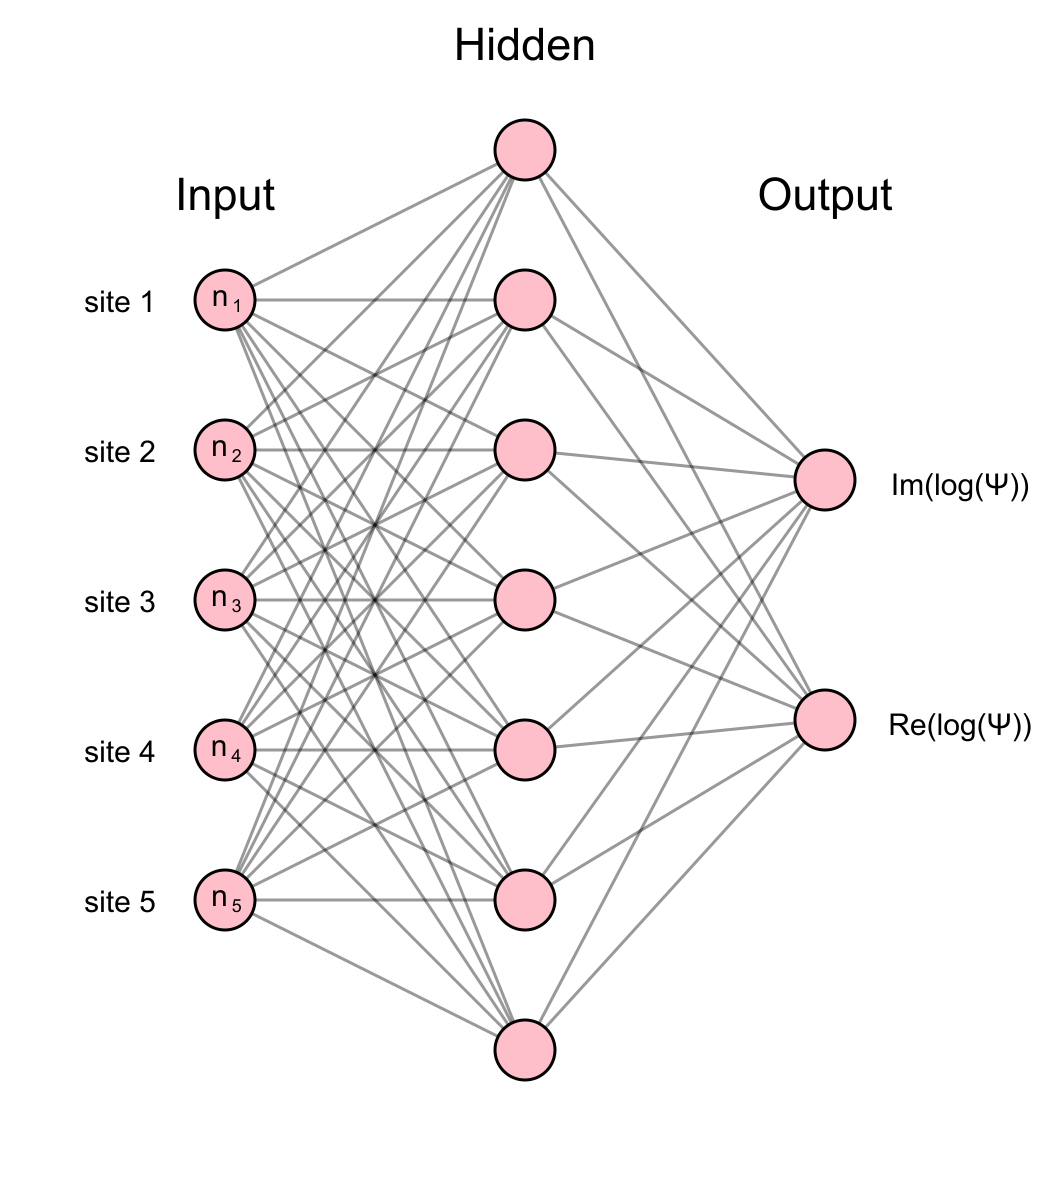
\includegraphics[width=\textwidth]{ch8/ANN.png}
    \end{subfigure}
    \caption{Pictorial representation of the neural network}
    \label{fig:ann}
\end{figure}
%%% FIG %%%
\FloatBarrier \!\!\!\!\!\!\!\!\!\!\!

We take a different approach here by utilizing a universal function approximator instead of any particular form of ansatz. In principle, a feed-forward neural network with sufficient hidden layers and nodes is capable of serving this purpose\cite{lu2020universal} such that the variational parameters are simply the network weights. Let us now consider the wavefunction of the Bose-Hubbard model with $N$ particles and $M$ lattice sites in the occupation basis.

\begin{equation}
    \ket{\Psi} = \sum_{\sum_i n_i = N }\psi(n_1, n_2, ..., n_M)\ket{n_1, n_2, \dots, n_M} = \sum \psi(\mathbf{n})\ket{\textbf{n}}
\end{equation}
The input layer of the network will have $M$ nodes, such that the basis state $\ket{\mathbf{n}} \equiv \ket{n_1, n_2, \dots, n_M}$ can be set as an input as shown in Fig. \ref{fig:ann}. The values of the nodes on the hidden layers are computed as usual, using a hyperbolic tangent activation function:
\begin{equation}
    u_j^{(0)} = n_j \hspace{1cm}; u_m^{(i+1)} = \sum_{k = 1}^{N_H^{(i)}}W_{mk}^{(i+1)}\tanh u_k^{(i)}(\mathbf{n}) + h_m^{(i+1)}
\end{equation}
The output layer will have 2 nodes such that we can get the co-efficient of the input basis state like so:
\begin{equation}
    \psi(\mathbf{n}) = \exp[u_1^{N_l}(\mathbf{n}) + iu_2^{N_l}(\mathbf{n})]
\end{equation}
The wavefunction can now be represented in this compact neural network once we tune the parameters, $\{W^{\mathbf{n}}, h^{\mathbf{n}}\}|_1^{N_l}$ by minimizing the energy. Generally, the expectation value of an operator, $\hat{A}$ is calculated using the expression:
\begin{equation}
    \langle A \rangle = \frac{\sum_{\mathbf{n}, \mathbf{n}'} \psi^*(\mathbf{n})\bra{\mathbf{n}}\hat{A}\ket{\mathbf{n}'}\psi(\mathbf{n}')}{\sum_\mathbf{n} |\psi(\mathbf{n})|^2}
\end{equation}
However, if we compute every element of the sum by retrieving the coefficients from our neural network, we effectively lose the benefit of having a compact representation. Instead, we utilize the standard Monte Carlo scheme, where the basis states are importance sampled, using the Metropolis algorithm. Since our goal is to sample states $\{n\}$ following the distribution $|\psi(\mathbf{n})|^2/\sum_{\mathbf{n}'}|\psi(\mathbf{n}')|^2$, we accept the proposal $\mathbf{n_1} \rightarrow \mathbf{n_2}$ with probability $|\psi(\mathbf{n_2})|^2/|\psi(\mathbf{n_1})|^2$ and compute the expectation value as follows.
\begin{equation}
    \left \langle \bra{\mathbf{n}}\hat{H}\ket{\mathbf{n}} \frac{\psi(\mathbf{n}')}{\psi(\mathbf{n})} \right \rangle_M \equiv \langle H \rangle_M    
\end{equation}
where $\langle\dots\rangle_M$ indicates an average over the metropolis sampling of $\mathbf{n}$. Training the network weights to represent the wavefunction requires us to perform a gradient descent.
\begin{equation}
    w \rightarrow w - \gamma \frac{\partial \langle \hat{H} \rangle_M}{\partial w}
\end{equation}
where, $\gamma$ is the learning rate, and the gradient can be computed using the following expression.
\begin{equation}
    \frac{\partial \langle \hat{H} \rangle}{\partial w} \approx 2\text{Re}(\langle O_w \hat{H}\rangle_M - \langle O_w^*\rangle_M\langle\hat{H}\rangle_M) \hspace{1cm} O_w(\mathbf{n}) = \frac{1}{\psi(\mathbf{n})}\frac{\partial \psi(\mathbf{n})}{\partial w}
\end{equation}
Further details can be found in Saito (2017) \cite{Saito_2017}. Our implementation can be found on \href{https://github.com/20akshay00/MSThesis}{github}, however, in its current state it is unusable due to inefficient computation of the gradient. This leads to extremely large runtimes for even small system sizes. Further, a naive gradient descent approach gets trapped in local minima even for the Bose-Hubbard model\cite{Saito_2017}. As a result, this line of exploration was not pursued further. It is worth noting, however, that there are larger and more mature projects that implement various machine learning techniques to solve many body problems, such as NetKet\cite{Vicentini_2022}.

\section{Stochastic Series Expansion}

We now turn to a class of extremely powerful methods that are broadly classified as Quantum Monte Carlo techniques. There are countless variations and flavors\cite{Pollet_2012, Austin2012} depending on the specifics of the system under consideration, but they all share the trait of utilizing Monte Carlo sampling in some capacity to solve quantum problems. We will focus on one flavor in particular, the stochastic series expansion (SSE)\cite{sandvik2019stochastic}. This section will largely follow the discussion presented in Sandvik's lecture notes\cite{Sandvik_2010}.
\vspace{0.5cm}\\
Generally, the goal of these methods is to compute the partition function and hence the thermal expectation values of various observables of interest. We begin by performing a Taylor expansion of the exponent around $\beta = 0$ and taking the trace with respect to an appropriate basis set $\{\alpha\}$.
\begin{equation}
    Z = \Tr{e^{-\beta H}} = \Tr{\sum_{n = 0}^{\infty} \frac{(-\beta)^n}{n!}H^n} = \sum_{\alpha} \sum_{n = 0}^{\infty} \frac{(-\beta)^n}{n!}\bra{\alpha}H^n\ket{\alpha}
\end{equation}
We can view the above sum as a Monte Carlo sampling of the configurations, $(\ket{\alpha}, n)$ with the weight, $W(\ket{\alpha}, n) = \frac{(-\beta)^n}{n!}\bra{\alpha} H^n \ket{\alpha}$. However, there is a glaring problem, that is the infinite sum over the expansion order, $n$. At first sight, such a situation seems impossible to deal with in a numerical algorithm. However, a solution presents itself if we analyze the nature of the energy and specific heat capacity calculated through this procedure.
\begin{align}\label{eq:mc_energy}
    \langle H \rangle &= \frac{1}{Z}\Tr{He^{-\beta H}} \nonumber\\
    &= \frac{1}{Z}\sum_{\alpha} \sum_{n = 0}^{\infty} \frac{(-\beta)^n}{n!}\bra{\alpha}H^{n+1}\ket{\alpha} \nonumber\\
    &= -\frac{1}{Z}\sum_{\alpha} \sum_{n = 1}^{\infty} \frac{n}{\beta} \cdot \frac{(-\beta)^n}{n!}\bra{\alpha}H^{n}\ket{\alpha} = \frac{\langle n \rangle}{\beta}
\end{align}
Similarly, we get $\langle H^2 \rangle = \langle n(n-1)\rangle/\beta^2$. The expression for the specific heat can then be computed as follows.
\begin{equation}
    C_v = \frac{\langle H^2 \rangle - \langle H \rangle^2}{T^2} = \langle n^2 \rangle - \langle n \rangle^2 - \langle n \rangle
\end{equation}
Generally, the specific heat vanishes as $T \to 0$ for quantum systems, so we can write $\sigma_n = \langle n^2 \rangle - \langle n \rangle^2 = \langle n \rangle$. Thus, we have $\langle n \rangle \sim N\beta$ and $\sigma_n \sim \sqrt{N\beta}$ where $N$ is the system size which is introduced since the energy roughly scales with the $N$. This tells us that the distribution of $n$ that contributes to the sum is quite narrow and we can simply introduce a cut-off length $L$ in our algorithm (that must be adjusted as the simulation progresses). 

%%% FIG %%%
\begin{figure}[!htb]
    \centering
    \begin{subfigure}[b]{0.75\textwidth}  %keep total sum <1 to show in same line
        \centering
        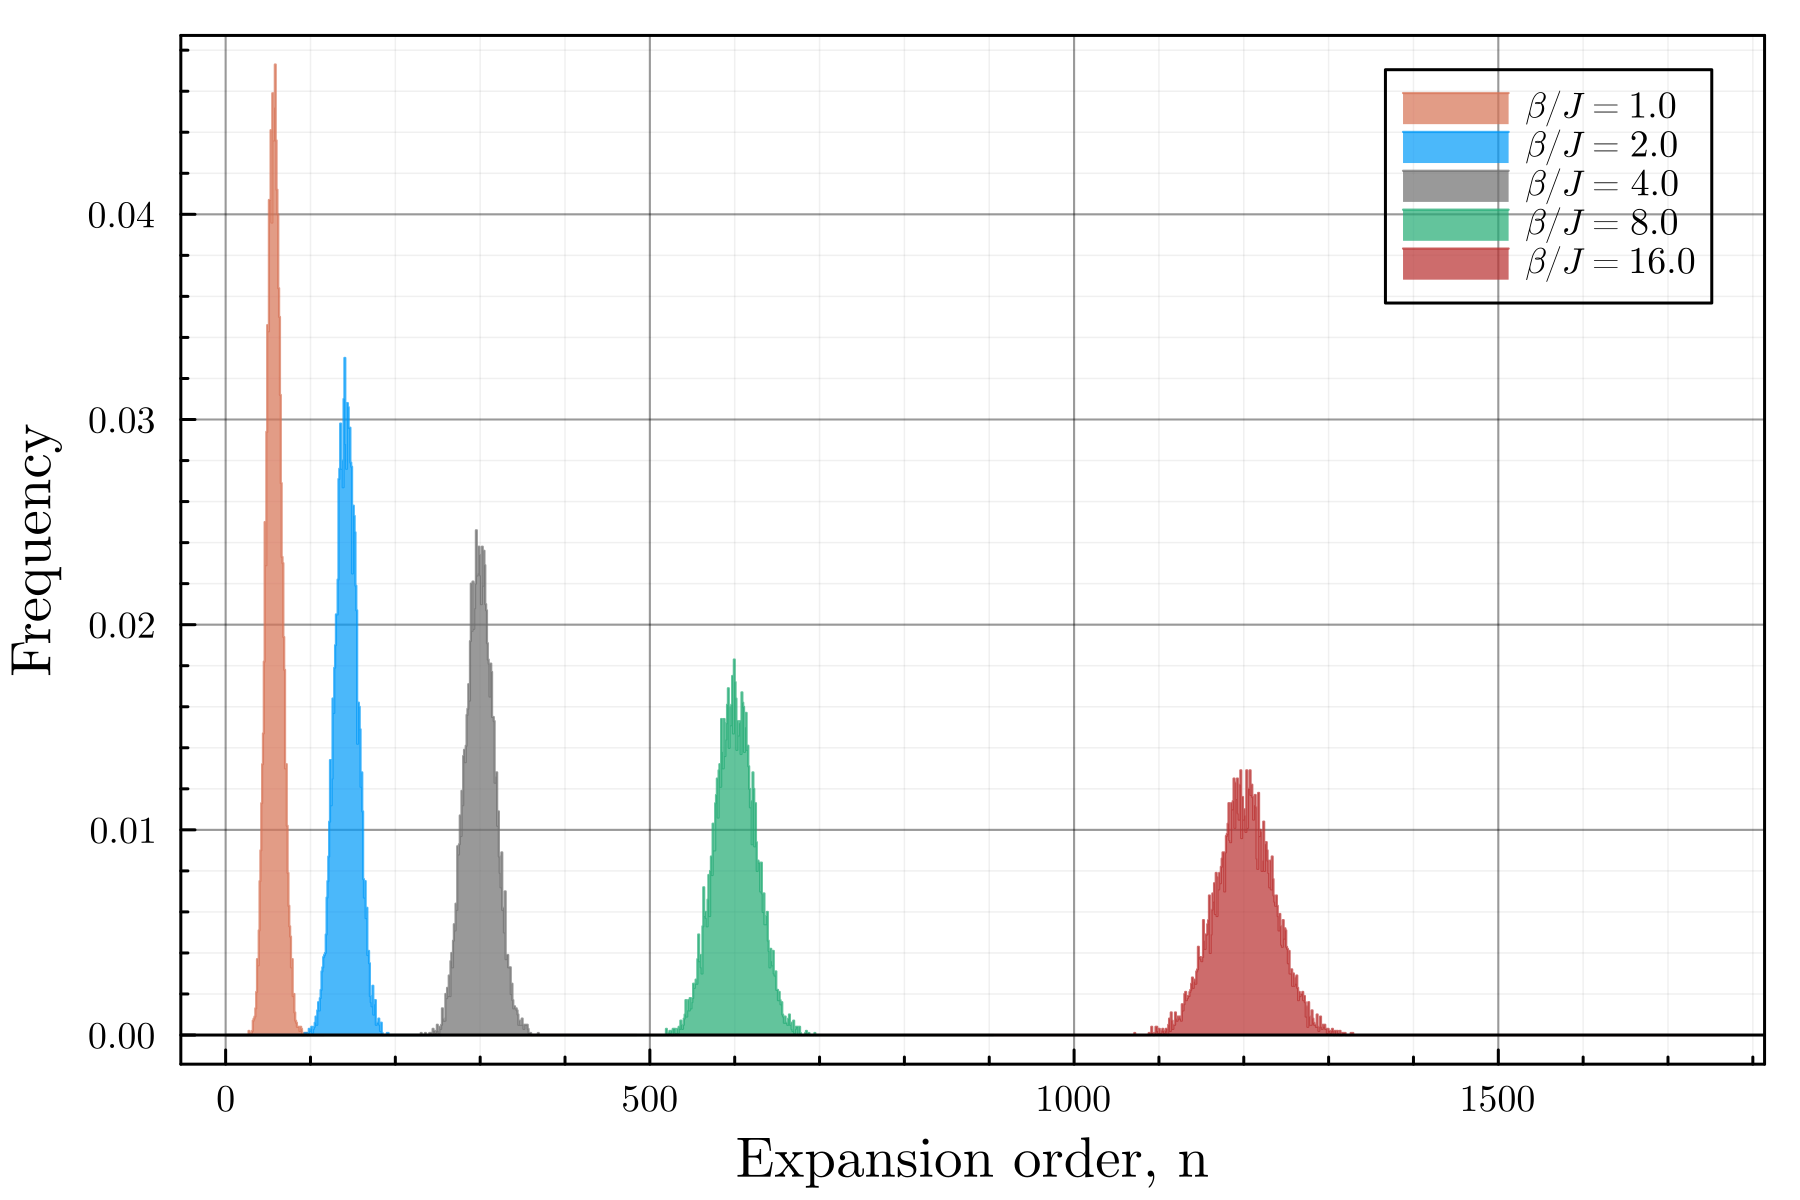
\includegraphics[width=\textwidth]{ch8/ndist.png}
    \end{subfigure}
    \caption{Distribution of expansion order in SSE}
    \label{}
\end{figure}
%%% FIG %%%
\FloatBarrier \!\!\!\!\!\!\!\!\!\!\!

\vspace{-0.5cm}
At this point, we note that computing the quantity $\bra{\alpha}H\ket{\alpha}$ is generally non trivial, and so we introduce an important idea that makes the SSE tractable. Generally, lattice Hamiltonians can be broken down as $H = -\sum_{a, b} H_{a, b}$, where $b$ indicates the "bond" connecting two sites $i(b)$ and $j(b)$, and $a$ indicates the class of the operator. Any power of the Hamiltonian can then be written in terms of a sum over 'operator strings' $\{H_{ab}\}$.
\begin{equation}
    (-H)^n = \sum_{\{H_{ab}\}} \prod_{p = 1}^n H_{a(p), b(p)}
\end{equation}
Putting this together with the fixed length scheme that was motivated above, we can write the partition function in the typical monte carlo format.
\begin{equation}
    Z = \sum_{\alpha, H_{ab}} \frac{\beta^n (L - n)!}{L!} \bra{\alpha}\prod_{p = 1}^n H_{a(p), b(p)}\ket{\alpha} \hspace{0.5cm} \leftrightarrow \hspace{0.5cm} Z = \sum_{C_i} W(C_i)    
\end{equation}

\begin{equation}
    \langle O \rangle = \frac{1}{Z}\sum_{\alpha, H_{ab}} \frac{\beta^n (L - n)!}{L!} \bra{\alpha}O\prod_{p = 1}^n H_{a(p), b(p)}\ket{\alpha} \hspace{0.5cm} \leftrightarrow \hspace{0.5cm} \langle A \rangle = \frac{\sum_{C_i} O(C_i)W(C_i)}{\sum_{C_i} W(C_i)}
\end{equation}
We have now introduced an abstract configuration which is a 2-tuple consisting of $\ket{\alpha}$, an element of the basis set, and $\{H_{ab}\}$ which is a string of $L$ bond operators. In order to work with the fixed-length scheme, we have also introduced $H_{0,0} = \mathbb{I}$ to pad the operator string, such that each string consists of $n$ non-identity bond operators and $(L-n)$ identities, thus sampling the expansion orders $n \in [1, L]$. 
\vspace{0.5cm}\\
The problem has now reduced to ergodically sampling this configuration space according to their weights (which can be computed with ease due to the bond decomposition). An issue arises when the weights are not positive, in which case they cannot be interpreted as probabilities, thus giving rise to the infamous \textit{sign problem}\cite{pan2022sign}. This is usually the case for fermionic systems and systems with non-bipartite lattices geometries. 

\subsection{S=1/2 Heisenberg model}
Let us now consider the spin-1/2 Heisenberg model with anti-ferromagnetic interactions ($J > 0$) on a square lattice. We choose this particular example since it is quite illustrative of the SSE technique while also having some relevance to the Bose-Hubbard model that we will discuss at the end of the chapter.  
\begin{equation}
    H = J\sum_{\langle i, j \rangle} S_i \cdot S_j
\end{equation}
A natural basis set to use in our expansion is the $S_z$-basis, $\ket{S_1^z, S_2^z, \cdots, S_N^z}$. We can now rewrite the Hamiltonian as a sum of bond operators:
\begin{equation}
    H_{1, b} = \frac{1}{4} - S_{i(b)}^z S_{j(b)}^z \hspace{1cm} H_{2, b} = \frac{1}{2}(S_{i(b)}^+ S_{j(b)}^- + S_{i(b)}^- S_{j(b)}^+)    
\end{equation}
\begin{equation}
    H = J\sum_{b = 1}^B [S_{i(b)}^z S_{j(b)}^z + \frac{1}{2}(S_{i(b)}^+ S_{j(b)}^- + S_{i(b)}^- S_{j(b)}^+)] = -J\sum_{b=1}^{N_B}(H_{1, b} - H_{2, b}) + \frac{JN_b}{4}
\end{equation}
Here, we have introduced two 'classes' of bond operators, that is, those that are diagonal ($H_{1, b}$) and off-diagonal ($H_{2, b}$) in the $S_z$-basis.
There is also an important restriction on the choice of the bond operators $H_{a,b}$, namely, that they must be non-branching, i.e, $H_{a,b}\ket{\alpha_i} = C_{a,b}^{i, j} \ket{\alpha_j}$ where $\ket{\alpha_i}$ and  $\ket{\alpha_j}$ are single elements of the chosen basis set. This implies that each configuration can equivalently be understood as a periodic sequence of basis elements (due to the cyclic nature of the trace).
\begin{equation}
    C \equiv \ket{\alpha_0} \rightarrow \ket{\alpha_1} \rightarrow \dots \rightarrow \ket{\alpha_{L-1}} \rightarrow \ket{\alpha_0} \hspace{1cm} \ket{\alpha_i} = \prod_{p=1}^iH_{a(p), b(p)}\ket{\alpha_0}
\end{equation}
Notice that we have also introduced a constant energy shift in order to force the matrix elements, and hence the configuration weights to be positive. Since the bond operators only act on two sites, we can list out all of these matrix elements:
\begin{align*}
    &\bra{\uparrow_{i(b)} \downarrow_{j(b)}}H_{1, b}\ket{\uparrow_{i(b)} \downarrow_{j(b)}} = \frac{1}{2}\hspace{1cm} \bra{\downarrow_{i(b)} \uparrow_{j(b)}}H_{2, b}\ket{\uparrow_{i(b)} \downarrow_{j(b)}} = \frac{1}{2} \\ 
    &\bra{\downarrow_{i(b)} \uparrow_{j(b)}}H_{1, b}\ket{\downarrow_{i(b)} \uparrow_{j(b)}} = \frac{1}{2} \hspace{1cm}     \bra{\uparrow_{i(b)} \downarrow_{j(b)}}H_{2, b}\ket{\downarrow_{i(b)} \uparrow_{j(b)}} = \frac{1}{2} 
\end{align*}
Note that any bond operator can only act on anti-parallel spins, since all other configurations have a vanishing matrix element. Further, we see that not only are the non-zero matrix elements positive but they are also equal. This greatly simplifies the algorithm, since the weight of any valid configuration is simply computed as follows.
\begin{equation}
    W(\alpha, \{H_{a, b}\}) = \left ( \frac{\beta}{2} \right )^n \frac{(L - n)!}{L!}
\end{equation}
The challenge now is to come up with a sampling scheme that generates operator strings that samples such periodic sequences of basis elements. There are usually three types of updates that are required to maintain ergodicity:
\begin{itemize}
    \item \textbf{Diagonal update:} This changes $n$, the number of non-identity bond operators in the operator string. Such an update simply replaces an identity operator with a diagonal one  (or vice versa) if the spin states it acts on is anti-parallel. 
    \item \textbf{Off-diagonal update: } Off-diagonal operators cannot be added or removed individually as was the case with the diagonal operators, since the periodicity of the basis state has to be preserved. As a result, one has to manipulate pairs of off-diagonal operators acting on the same sites, however such an update scheme is quite inefficient. Instead, another approach known as the operator loop update\cite{Sandvik_1999} is used wherein a loop is constructed across the entire configuration, connecting the spin sites at the base of several operators, which are then flipped simultaneously in an analogous manner to the cluster updates in the Ising model. This scheme is related to a broader class of loop algorithms\cite{evertz2003} applicable to general quantum monte carlo methods.
    \item \textbf{Spin-flip update: } Finally, if a particular spin is not acted upon by any operators, it can be flipped to sample a different basis state $\ket{\alpha}$. However, this update is not strictly required nor efficient since the off-diagonal updates already sample the basis states as well.
\end{itemize}

The probability of accepting these updates can then be computed by means of the usual constraint arising from detailed balance of the markov chain of configurations.
\begin{equation}
    P_{\text{accept}}(A \to B) = \min \left (\frac{W(B)P_{\text{select}}(B \to A)}{W(A)P_{\text{select}}(A \to B)}, 1\right )
\end{equation}
The interested reader may find the details of the sampling scheme as well as an ingenious way to visualize and implement the SSE in Sandvik's lecture notes\cite{Sandvik_2010}. 
\vspace{0.5cm}\\
Once we are able to sample the configurations ergodically, diagonal observables can be computed easily as they do not alter the sequence of basis states. On the other hand, off-diagonal observables are quite hard to compute, in general. However, any off-diagonal operator, $H_{2, b}$, which is a part of the Hamiltonian is found to be related to the expectation value of the number of occurences of the operator in the operator string\cite{Sandvik_2010}. For example, this is what we found for the energy in Eq. \eqref{eq:mc_energy}. Luckily, most of the observables that are required for our purposes fall within these two categories.

\subsection{Results}
We have performed the SSE for various lattice sizes and temperatures, recording $n=10000$ samples for computing each quantity. The results are shown as in Fig. \ref{fig:sse_res}. Although there are strong finite-size effects in most of the plots, we can see for $L=48$ that the (staggered) magnetization seems to undergo a transition somewhere between $J \cdot T \in [0.2, 0.6]$ indicating a shift from an anti-ferromagnet to a paramagnet. Peculiarly, the magnetic susceptibility $\chi$ seems to also have a continuous transition around the same region instead of a divergence as expected from a second order transition. On the other hand, we have some hint of divergence from the specific heat plot around $J\cdot T \approx 0.6$. 

%%% FIG %%%
\begin{figure}[!htb]
    \centering
    \begin{subfigure}[b]{\textwidth}  %keep total sum <1 to show in same line
        \centering
        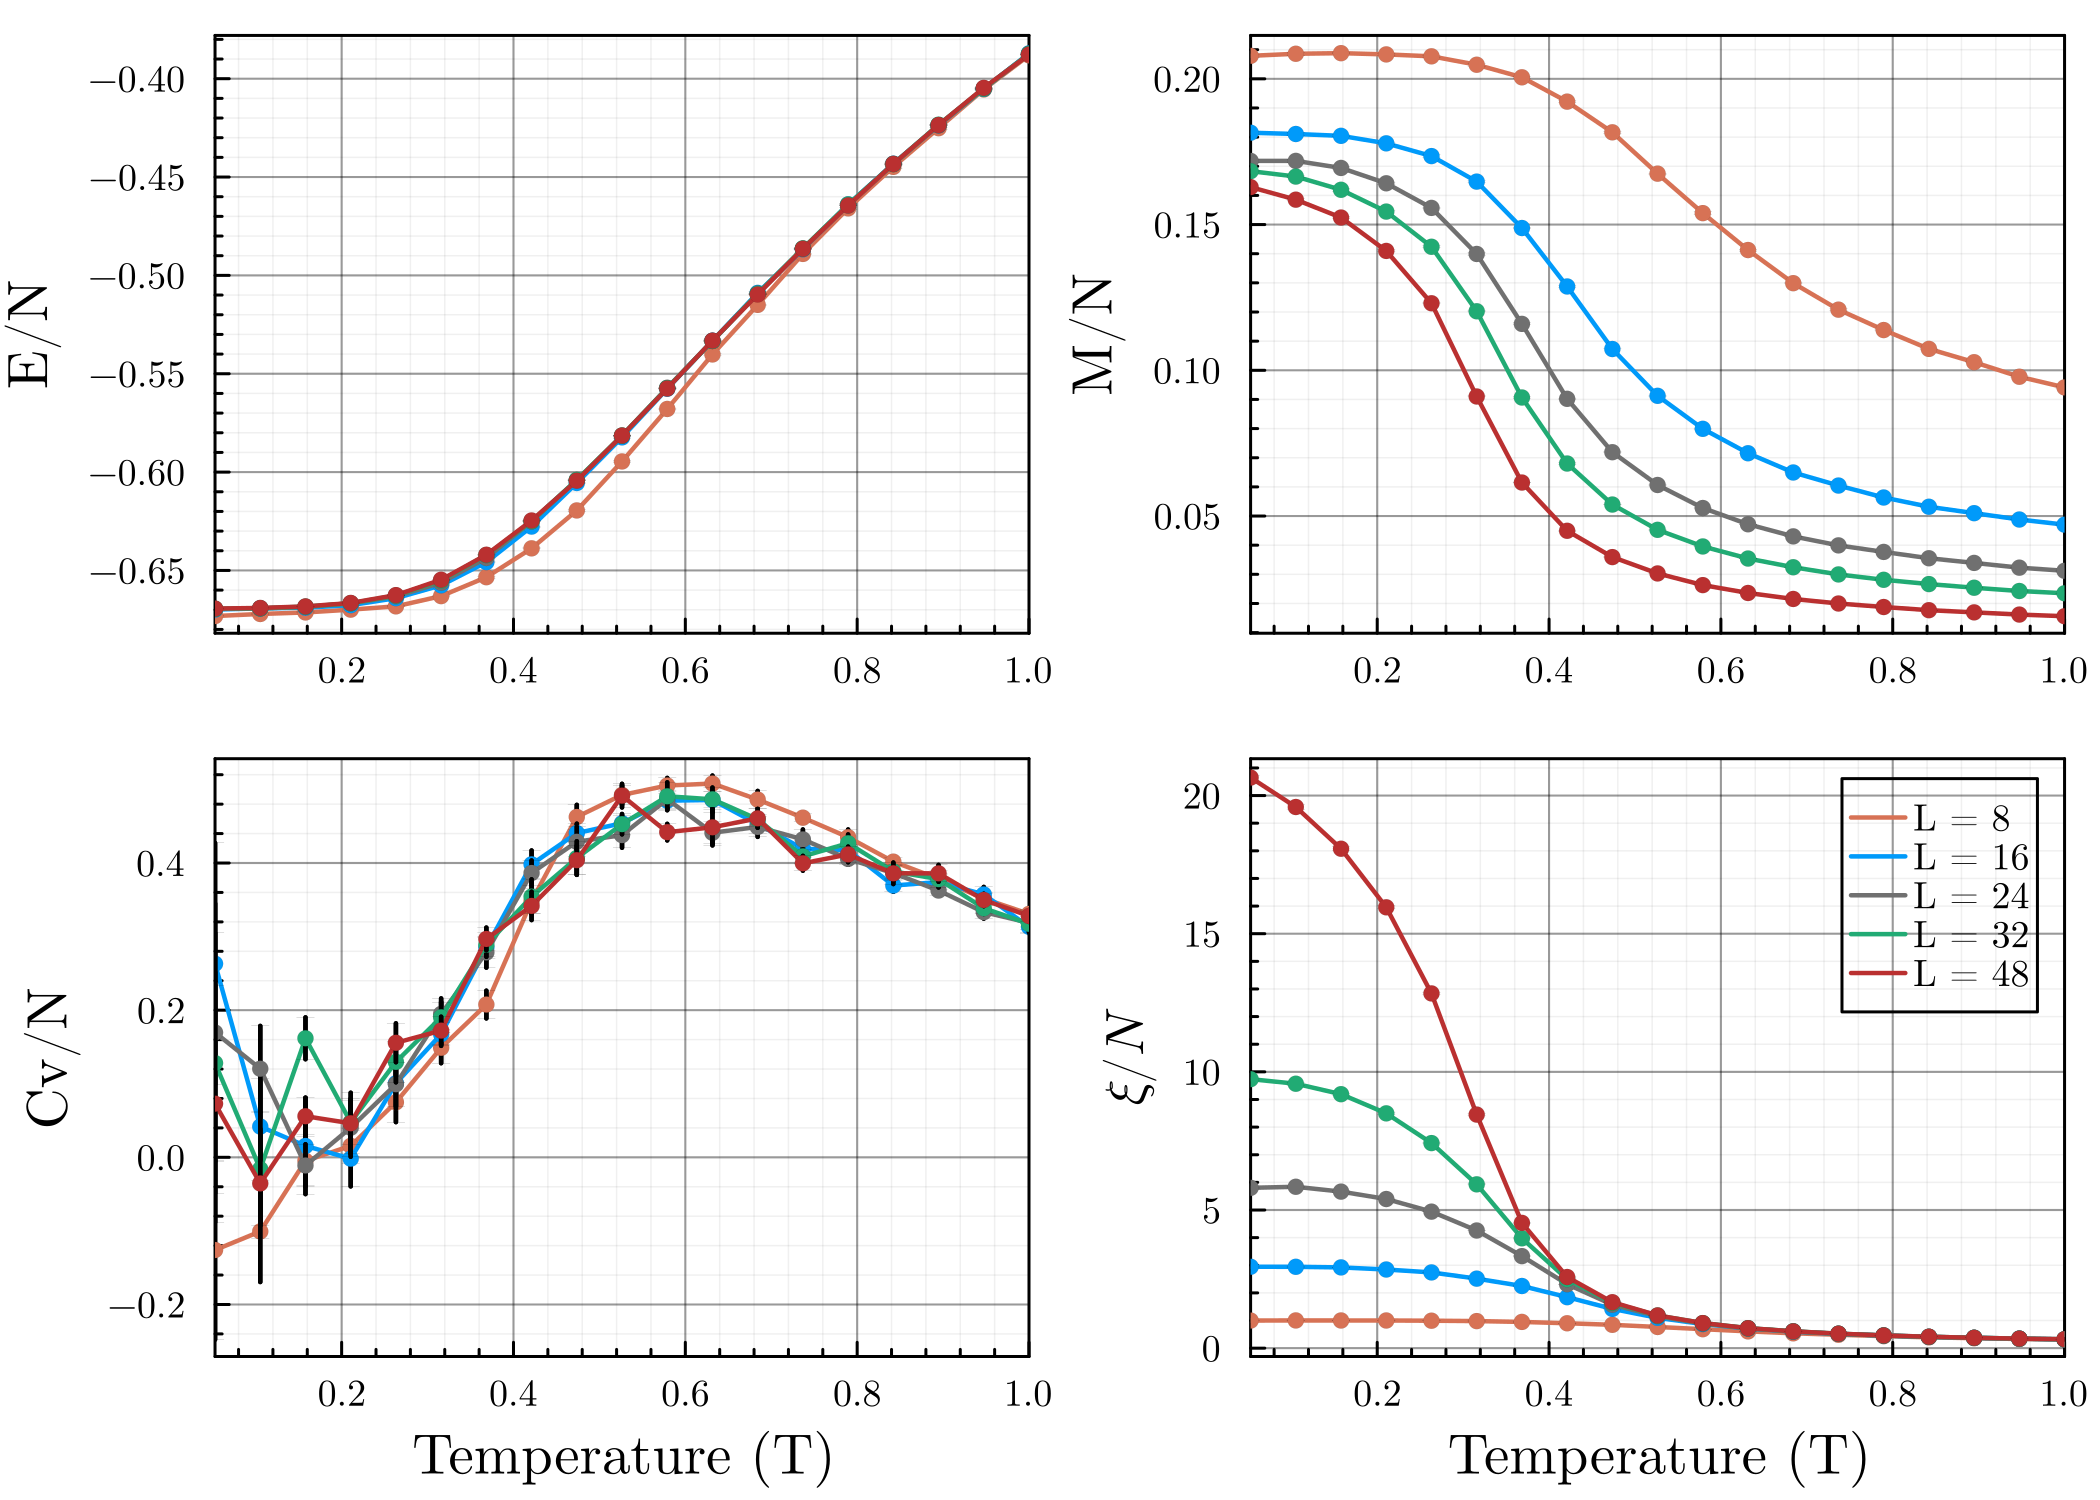
\includegraphics[width=\textwidth]{ch8/sse_stats.png}
    \end{subfigure}
    \caption{Tracking various quantities calculated using SSE}
    \label{fig:sse_res}
\end{figure}
%%% FIG %%%
\FloatBarrier \!\!\!\!\!\!\!\!\!\!\!

In order to extract a better estimate of the critical temperature by dealing with the finite size effects, we calculate the Binder cumulant for various lattice sizes in Fig. \ref{fig:sse_bc}. 
\begin{equation}
    U_L = 1 - \frac{\langle M^4 \rangle_L}{3\langle M^2 \rangle^2_L}
\end{equation}

%%% FIG %%%
\begin{figure}[!htb]
    \centering
    \begin{subfigure}[b]{\textwidth}  %keep total sum <1 to show in same line
        \centering
        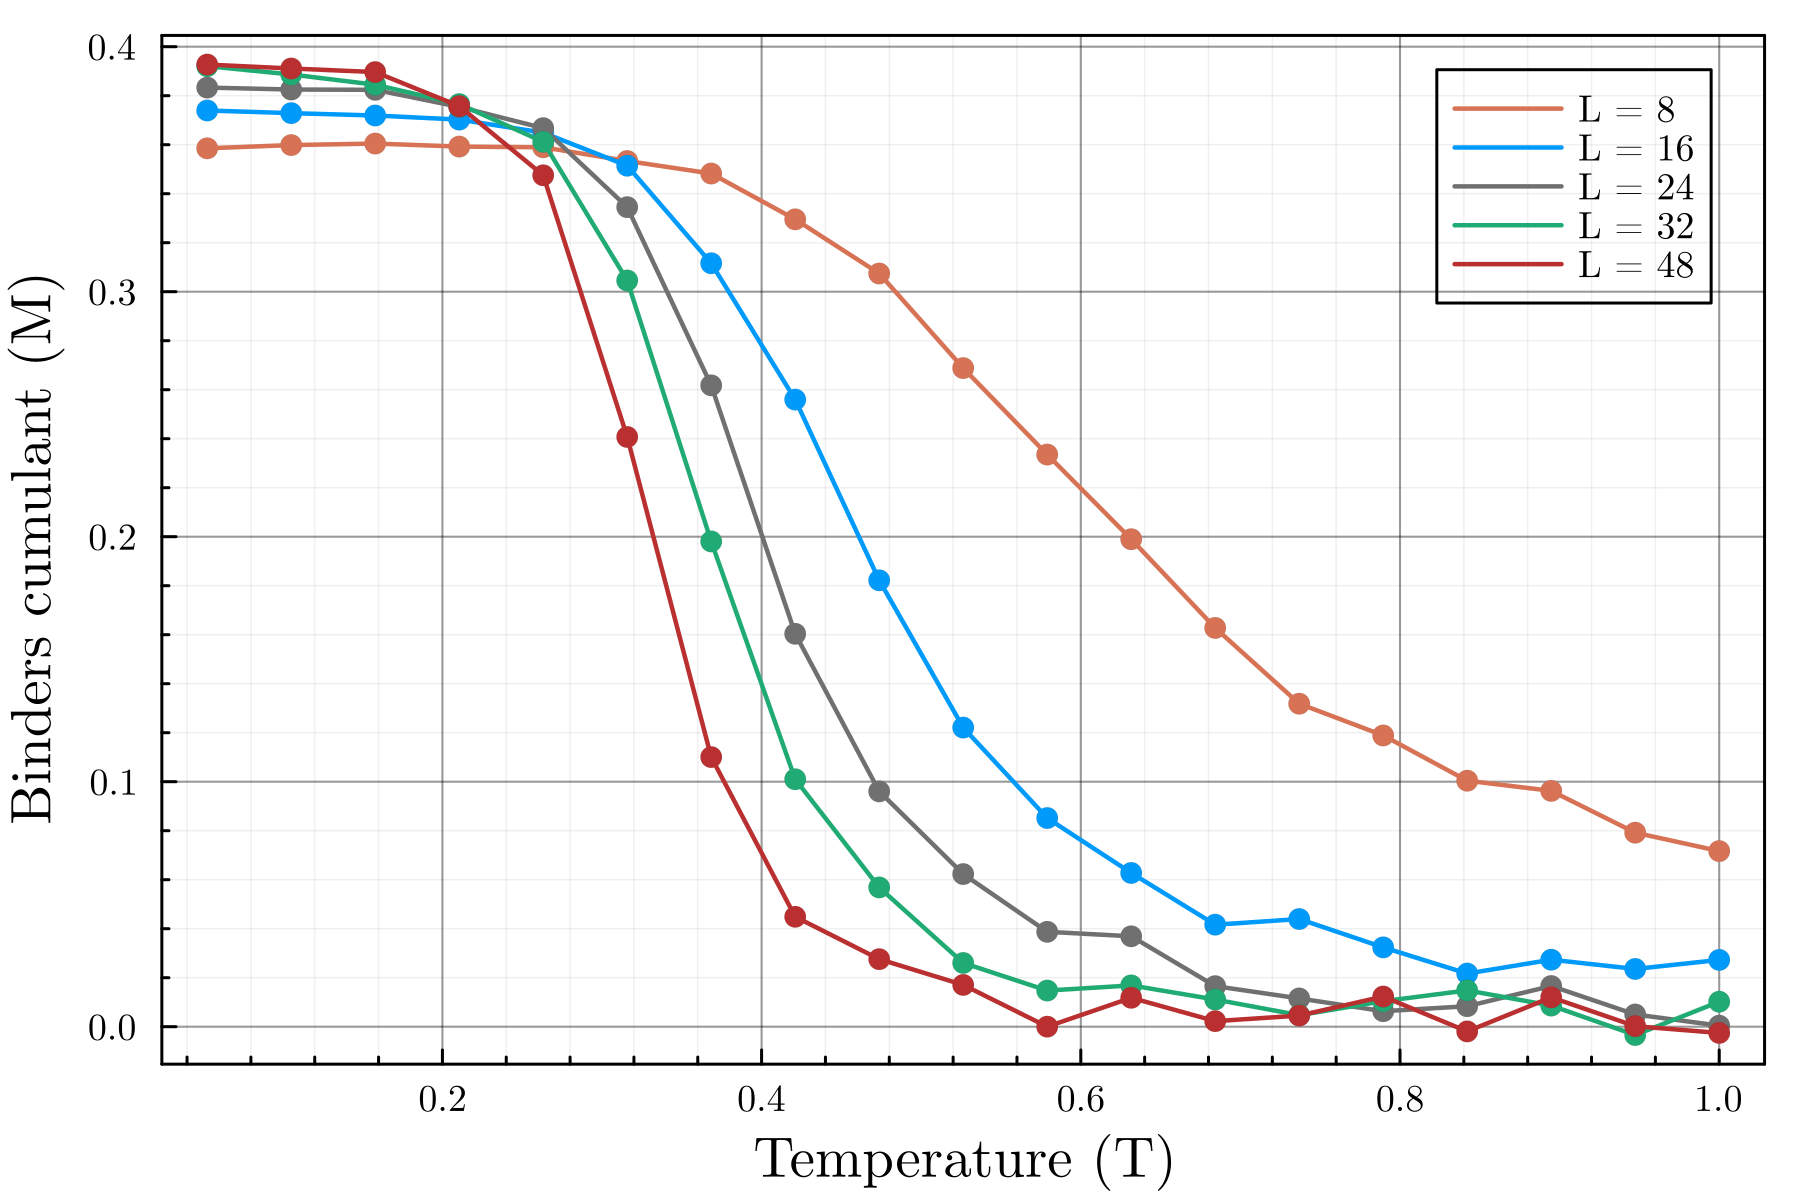
\includegraphics[width=0.75\textwidth]{ch8/sse_binder.png}
    \end{subfigure}
    \caption{Binder cumulant curves for various lattice sizes}
    \label{fig:sse_bc}
\end{figure}
%%% FIG %%%
\FloatBarrier \!\!\!\!\!\!\!\!\!\!\!

\vspace{-0.3cm}
We see that the curves roughly intersect at $J\cdot T \approx 0.22$. As it stands, these results significantly contradict with each other and we have not been able to resolve this so far. 

\subsection{Mapping to bosons}
The discussion so far seems rather unrelated to the rest of the thesis, however, a closer look at the Heisenberg Hamiltonian reveals that this is not the case:
\begin{equation}
    H = J\sum_{\langle i, j \rangle} \vec{S}_i \cdot \vec{S}_j = J\sum_{\langle i, j \rangle} \left [\frac{1}{2}(S_i^+ S_j^- + S_i^- S_j^+) +  S_i^z S_j^z \right ]
\end{equation}
Consider the mapping $S^+_i \to a_i^{\dagger}$, $S_i^- \to a_i$ and $S^z_i = n_i - 1/2$. The Hamiltonian is then oddly reminiscent of the extended Bose-Hubbard model.
\begin{equation}
    H = \frac{J}{2} \sum_{\langle i, j \rangle}(a_i^{\dagger}a_j + a_j^{\dagger}a_i) + J \sum_{\langle i, j \rangle} n_i n_j
\end{equation}
where $t = -J/2$ and $V = J$. Note that the on-site interaction term is missing. This is because we have effectively mapped classical spin-1/2 particles to hardcore bosons, i.e, in the limit of $U \to \infty$ s.t. $\langle n_i \rangle \in \{0, 1\}$. Loosely we can think of states having $\langle S^z \rangle = -1/2$ and $\langle S^z \rangle = 1/2$ corresponding to $\langle n \rangle = 0$ and $\langle n \rangle = 1$ boson occupation, respectively. Note that the $a^{\dagger}$ ($a$) operators here are not general bosonic operators, but specifically ones that create (annihilate) hard-core bosons.

%%% FIG %%%
\begin{figure}[!htb]
    \centering
    \begin{subfigure}[b]{\textwidth}  %keep total sum <1 to show in same line
        \centering
        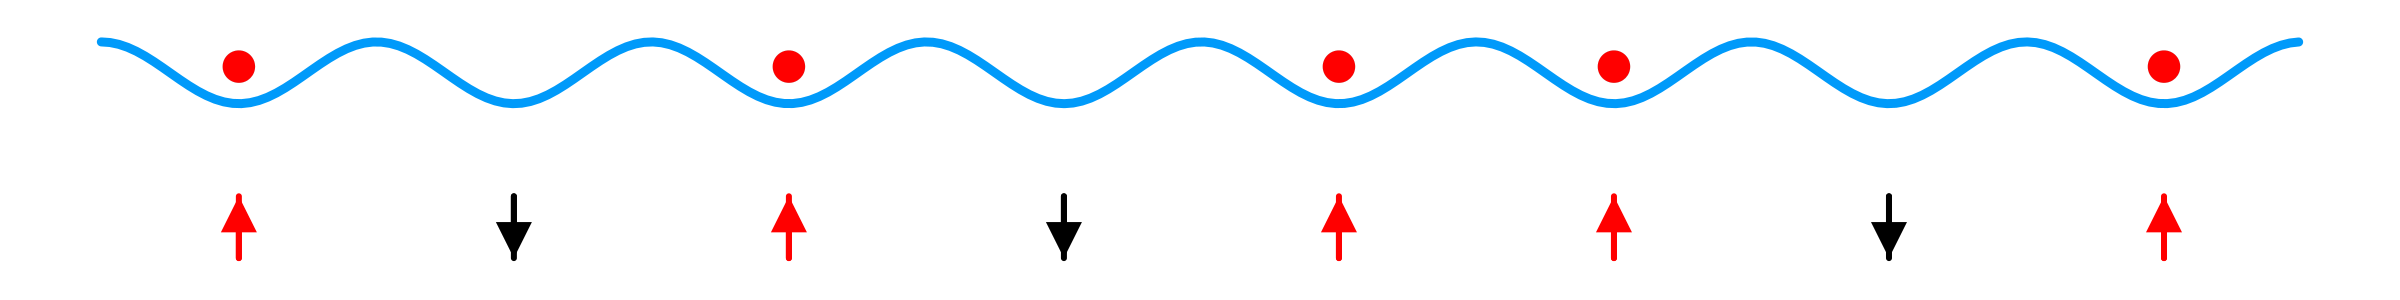
\includegraphics[width=\textwidth]{ch8/bosonspin.png}
    \end{subfigure}
    \caption{Mapping hard-core bosons to classical spin-1/2 particles}
    \label{}
\end{figure}
%%% FIG %%%
\FloatBarrier \!\!\!\!\!\!\!\!\!\!\!

In the most general case, we can map a spin-S anisotropic XXZ model to a semi-hardcore extended Bose-Hubbard model with maximum occupation of $2S$.

\begin{minipage}{0.7\textwidth}
\begin{align*}
    H &= J_x\sum_{\langle i, j \rangle} (S_i^+ S_j^- + S_i^- S_j^+) +  J_z\sum_{\langle i, j \rangle} S_i^z S_j^z + h_z \sum_i S_i^z\\
    H &= -t \sum_{\langle i, j \rangle}(a_i^{\dagger}a_j + a_j^{\dagger}a_i) + V \sum_{\langle i, j \rangle} n_i n_j - \mu \sum_i n_i
\end{align*}    
\end{minipage}
\begin{minipage}{0.25\textwidth}
    \begin{align*}
        t &\equiv J_x \\
        V &\equiv J_z \\ 
        \mu &\equiv J_z - h_z
    \end{align*}
\end{minipage}

However, in such a case, there are many more non-zero matrix elements that exist which are also not necessarily equal in magnitude. As a result, the operator loop update has to be redesigned since there is no unique deterministic loop that can be constructed for a given configuration. This can be remedied by utilizing the directed loop algorithm\cite{Syljusen_2002} which applies to the most general situations. 
\vspace{0.5cm}\\
Our implementation of the SSE for the isotropic spin-1/2 Heisenberg model can be found on \href{https://github.com/20akshay00/MSThesis}{github}. Although we intended to implement the directed loop algorithm as well, we were unable to do so within the constraint of the thesis and will not discuss its details here. 

\section{World-line QMC}
While the SSE is quite straightforward conceptually, it can efficiently generate samples only when the diagonal and off-diagonal terms are of comparable magnitude\cite{Sandvik_2010} ($t \sim U, t \sim V$ for e.g.). This is generally satisfied for spin systems, however, the interesting regions in bosonic systems occur for $t \ll U, t \ll V$. As a result, the SSE sampling scheme is not the best choice for our purposes. Instead, we turn to a related class of algorithms loosely termed as world-line QMC\cite{schneider2008}. We first discuss the discrete formulation.
\begin{equation}
    Z = \Tr{e^{-\beta H}}  = \Tr{\prod_{l = 1}^L e^{-\Delta\tau H}} \hspace{1cm} \Delta \tau = \beta/L
\end{equation}
Instead of expanding the exponential as a Taylor series, we utilize a Trotter decomposition to cast the sum in terms of the usual monte carlo language by inserting completeness relations of our prefered basis set, $\{\alpha \}$. We then have:
\begin{equation}
    Z = \sum_{\alpha_0}\sum_{\alpha_1}\dots\sum_{\alpha_L - 1} \bra{\alpha_0}e^{-\Delta\tau H}\ket{\alpha_{L-1}}\dots \bra{\alpha_2}e^{-\Delta\tau H}\ket{\alpha_1}\bra{\alpha_1}e^{-\Delta\tau H}\ket{\alpha_0}
\end{equation}
\begin{equation}
    Z \approx \sum_{\{\alpha\}}\bra{\alpha_0}1 - \Delta \tau H \ket{\alpha_{L-1}}\dots \bra{\alpha_2}1 - \Delta \tau H \ket{\alpha_1}\bra{\alpha_1}1 - \Delta \tau H \ket{\alpha_0}
\end{equation}
where, the error falls of as $\mathcal{O}(\Delta \tau)$ and vanishes in the limit $\Delta\tau \to 0$. The configurations here are quite similar to the idea we introduced in the SSE involving a cyclic sequence of basis states. While the diagonal parts of $H$ leave the basis state unaltered, the off-diagonal ones do not. Effectively, we can view this procedure as having introduced a new dimension, $\Delta \tau$ to our system. 
\vspace{0.5cm}\\
In principle, since the results of the above method are only exact when $\Delta \tau \to 0$, we must perform the simulation for various values of $\Delta \tau$ and extrapolate them to get the exact results. However, it turns out that such a technique is unnecessary as we can, infact, take the limit exactly to formulate a continuous time world-line approach\cite{schneider2008}. 
\begin{equation}
    Z = \Tr{e^{-\beta H}} = \Tr{\mathcal{T} e^{\beta H_0} \exp{-\int_0^{\beta} d\tau V(\tau)}}
\end{equation}
where, $V(\tau) = e^{\tau H_0}Ve^{-\tau H_0}$. The exponential can be expanded iteratively like so:
\begin{equation}
    Z = \Tr{e^{-\beta H_0} \sum_{n = 0}^{\infty} \int_0^{\beta} d\tau_1 \int_0^{\tau_1}d\tau_2\dots\int_0^{\tau_{n-1}} V(\tau_1)\dots V(\tau_n)}
\end{equation}
By inserting basis sets between the elements, this formulation becomes quite similar to the discrete case, except that the $d\tau$ dimension is now continuous. However, a naive sampling of these configurations would result in critical slowing down near the phase boundaries (among other issues)\cite{Prokofev1998}. There exists an analog of the directed loop updates for the continuous-time world-line approach, called the worm algorithm\cite{prokofev2010worm, Pollet_2007, sadoune2022efficient} which solves this issue. We intend to utilize this technique in our future studies to obtain more quantitative results.


% Choosing a relevant basis set $\{\ket{\alpha_i}\}$, we can then insert completeness relations to break down the expression for the partition function. 
% $$Z = \sum_{n=0}^{\infty} \frac{(-\beta)^n}{n!}\sum_{\{\alpha\}_n} \bra{\alpha_0}H\ket{\alpha_{n-1}}\dots\bra{\alpha_2}H\ket{\alpha_1}\bra{\alpha_1}H\ket{\alpha_0}$$

% The expectation value of the Hamiltonian can then be written like so:
% \begin{align*}
%     E &= \langle H \rangle = \frac{1}{Z}\Tr{He^{-\beta H}}\\
%      &= \frac{1}{Z}\sum_{n=0}^{\infty} \frac{(-\beta)^n}{n!}\sum_{\{\alpha\}_{n+1}} \bra{\alpha_0}H\ket{\alpha_{n+1}}\dots\bra{\alpha_2}H\ket{\alpha_1}\bra{\alpha_1}H\ket{\alpha_0}    \\
%      &= -\frac{1}{Z}\sum_{n=1}^{\infty} \frac{(-\beta)^n}{n!} \cdot \frac{n}{\beta} \cdot \sum_{\{\alpha\}_n} \bra{\alpha_0}H\ket{\alpha_n}\dots\bra{\alpha_2}H\ket{\alpha_1}\bra{\alpha_1}H\ket{\alpha_0}  = \frac{\langle n \rangle}{\beta}   
% \end{align*}